\documentclass[12pt]{beamer}

% ****************
% ***** INFO *****
% ****************
\usepackage[english]{babel}
\title[]{The Effect Of The Minimum Wage When It Really Bites: A Reexamination Of The Evidence From Puerto Rico}
\subtitle{ECAG-6665: Research Report}
\author[Name Surname]{Alejandro Ouslan}
\institute[institute]{University of Puerto Rico}
\date{} % or \today

% *******************
% ***** PROJECT *****
% *******************
% main color: to black
\definecolor{main}{HTML}{000000}
\setbeamercolor{structure}{fg=main}

% *****************
% ***** THEME *****
% *****************
\usepackage{helvet}
\renewcommand{\familydefault}{\sfdefault}
\setbeamertemplate{frametitle continuation}{\gdef\beamer@frametitle{}}
\setbeamertemplate{footline}{}
\setbeamertemplate{navigation symbols}{}
\usepackage{csquotes}
\usepackage[backend=biber,style=numeric]{biblatex}
\addbibresource{reference.bib} % Link to the bibliography file

% *****************
% ***** CODE *****
% *****************
\usepackage{listings}
\lstdefinestyle{py}{
	backgroundcolor=\color{white},
	basicstyle=\ttfamily\scriptsize,
	breaklines=true,
	commentstyle=\color{gray},
	keywordstyle=\color{blue},
	stringstyle=\color{magenta},
	language=Python
}

% **********************
% ***** ALGORITHMS *****
% **********************
\usepackage{algorithm}
\usepackage{algpseudocode}

% *****************
% ***** UTILS *****
% *****************
\usepackage{xcolor}

% ********************
% ***** DOCUMENT *****
% ********************
\begin{document}

% **********************
% ***** TITLEPAGE ******
% **********************
\begin{frame}{}
	\vspace{\fill}

	
\includegraphics[width=0.16\linewidth]{../../assets/uprm_logo.png}

	\vspace{\fill}

	\Large
	\color{main}
	\inserttitle

	\medskip

	\large
	\color{black}
	\insertsubtitle

	\vspace{\fill}

	\footnotesize
	\insertinstitute

	\vspace{\fill}

	\textbf{Author:} \insertauthor

	\medskip

	\insertdate

	\vspace{\fill}
\end{frame}

% *****************
% ***** START *****
% *****************
\begin{frame}[allowframebreaks]{Research Question}
	\begin{itemize}
		\item This paper reinvestigates the evidence on the impact of the minimum wage on employment in Puerto Rico. \cite{krueger1994effect}
	\end{itemize}

\end{frame}

\begin{frame}[allowframebreaks]{Justification of Research}
	\begin{itemize}
		\item Sectors that are forced to raise wages in response to a minimum should reduce employment because of both substitution
		      and scale effects.
		\item The recent wave of studies that conclude the minimum wage has not had an adverse impact on employment are somehow wrong.
		\item The minimum wage has the predicted effect when it is really high relative to the equilibrium wage.
	\end{itemize}

\end{frame}

\begin{frame}[allowframebreaks]{Literature Review}
	\begin{itemize}
		\item The spike in wage distribution at the minimumm wag eis an indication that people with presumablyu different ability levels earn the same wage. \cite{brown1988minimum}
		\item Case studies find that employment did not decline at establishments that were forced to race wages by the minimum compard to others that were not \cite{card1993minimum}
		\item The employment increased in restaurants that were forced to raise their wages to meet the new minimum wage in the short run \cite{card1992using}
	\end{itemize}

\end{frame}

\begin{frame}[allowframebreaks]{Data Characteristics and Data Sources}
	\begin{itemize}
		\item The data comes from Yearbook of Labor Statistics
	\end{itemize}
\end{frame}

\begin{frame}[allowframebreaks]{Methodology}
	\begin{itemize}
		\item Esimating an employment demand equation
		      \begin{equation}
			      \frac{\partial X}{.5(X_0 + X_1)} - \frac{d N}{.5(N_0 + N_1)} = \alpha + \beta \frac{d W}{.5(W_0 + W_1)}
		      \end{equation}
		\item The bias will be greater if profits and capital payments are small
		      \begin{equation}
			      \log{X_1/X_0} - \log{N_1/N_0} = \alpha + \beta \log{W_1/W_0}
		      \end{equation}
		\item The analysis ais a cross-industry panel data analysis of employment.
		      \begin{equation}
			      \log{EMP_{it}} = \alpha + \beta \log(c_{it}m_{it}/w_{it}) + T_i + IND_i + \epsilon_{it}
		      \end{equation}
	\end{itemize}

\end{frame}

\begin{frame}[allowframebreaks]{Results Figures}
	\begin{center}
		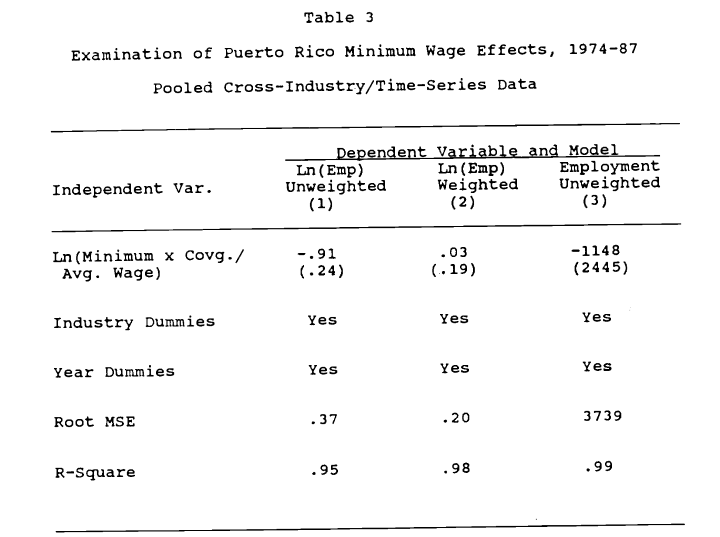
\includegraphics[width=0.8\linewidth]{assets/results.png}
	\end{center}
\end{frame}

\begin{frame}[allowframebreaks]{Descriptive Statistics}
	\begin{center}
		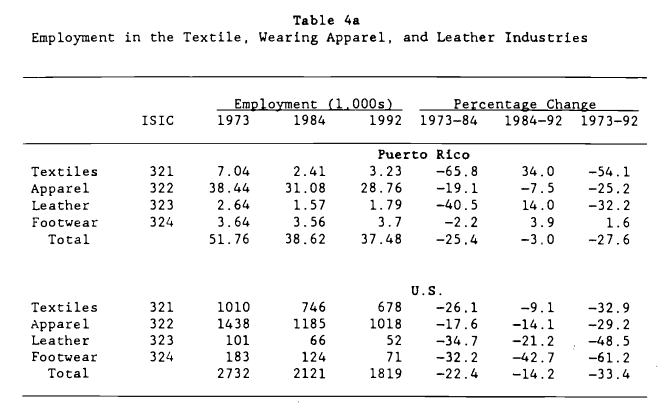
\includegraphics[width=0.8\linewidth]{assets/descriptive.png}
	\end{center}
\end{frame}

\begin{frame}[allowframebreaks]{Results}
	\begin{itemize}
		\item Between 1973 and 1984 employment declined by 66\% in textiles, by 19\% in apparel, and by 41\% in leather products.
		\item Between 1973 and 1984,the combined employment in these industries on the mainland fell by 600,000 jobs, or 22 percent of the initial level.
		\item Between 1973 and 1992, employment in these industries declined by more in the mainland than in PR.
	\end{itemize}
\end{frame}

\begin{frame}[allowframebreaks]{Graphs}
	\begin{center}
		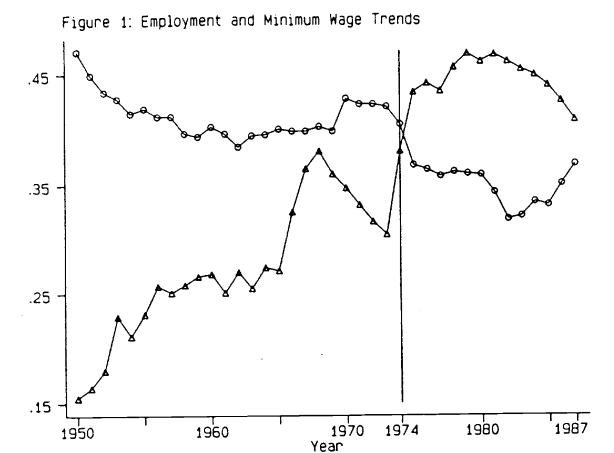
\includegraphics[width=0.8\linewidth]{assets/graph.png}
	\end{center}
\end{frame}

\begin{frame}[allowframebreaks]{Conclusions}
	\begin{itemize}
		\item The evidence of adverse employment effects of Puerto Rico's minimum wage is fragile and inconclusive.
		\item Strongest evidence: Aggregate time series analysis suggests a negative effect on employment.
		\item Weakest evidence: Cross-industry analyses show limited support for negative effects.
		\item An intelligent skeptic would likely remain unpersuaded by the evidence.
		\item Economists should explore alternative models to explain limited or nonexistent adverse effects.
	\end{itemize}
\end{frame}
% ************************
% ***** BIBLIOGRAPHY *****
% ************************
\begin{frame}[allowframebreaks]{Bibliography}
	\printbibliography
\end{frame}
% ***************
% ***** END *****
% ***************

\end{document}
